\documentclass{beamer}
\usepackage{tabularx}
\mode<presentation>
{
  %\usetheme{Warsaw}
  % or ...
  \usecolortheme{beaver}

  \setbeamercovered{transparent}
  % or whatever (possibly just delete it)
}

\title{ADPLL Network on an FPGA}
\author{Conor Dooley}
\subtitle{Semester 1 Presentation}

\begin{document}

\begin{frame}
    \titlepage
\end{frame}

\section*{Background Information}
\begin{frame}{Motivation}
  % - A title should summarize the slide in an understandable fashion
  %   for anyone how does not follow everything on the slide itself.

    \begin{itemize}
        \item[--]
            Clock source for System-On-Chip devices.
        \item[--]
        	While transistor count has risen, clock frequency has not.
        \item[--]
        	Want a low power clocking system that is suited to high frequency.
        \item[--]
            Goals of clocking system:
            \begin{itemize}
            	\item[]
            		Deliver in-phase clock signal to all parts of chip.
		        \item[]
		            Aim is to avoid synchronisation issues.
		    \end{itemize}
        \item[--]
            Why are synchronisation errors bad?
        \begin{itemize}
        	\item[]
        		De-sync between registers may reduce time for processing.
            \item[]
                As such forced to do less complex operations per clock cycle.
            \item[]
                Therefore must lower clock freq. or reduce complexity per cycle.
        \end{itemize}
    	\item[--]
    		Characterise this de-sync using:
    		\begin{itemize}
    			\item[]
    				Average value \textit{skew}.
    			\item[]
	    			Random process \textit{jitter}.
    		\end{itemize}
    \end{itemize}
 
\end{frame}

\begin{frame}{Existing Solutions}
  % - A title should summarize the slide in an understandable fashion
  %   for anyone how does not follow everything on the slide itself.
	\begin{columns}
		\column{0.55\linewidth}
		\textbf{Branch, H, X trees}
		\begin{itemize}
			\item[--]
				Use buffers to distribute in sync clock.
			\item[--]
				Rely on symmetry of delay.
			\item[--]
				This global matching is very challenging in large chips.
			\item[--]
				Suffer from fabrication mismatch problems.	
			\item[--]
				Solutions to mismatches further drive up power consumption.
			%\item[--]
			%	Leads to skew/jitter at high frequency. %TODO what leads to this?
		\end{itemize}
		\textbf{Clock Mesh}
		\begin{itemize}
			\item[--]
				Great timing accuracy.
			\item[--]
				Redundant high capacitance lines lead to large power consumption.
		\end{itemize}
		\column{0.45\linewidth}
			%\centering	
			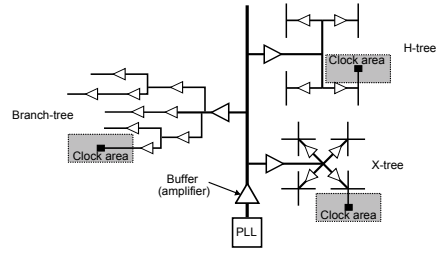
\includegraphics[scale=0.4]{eldar_trees}
			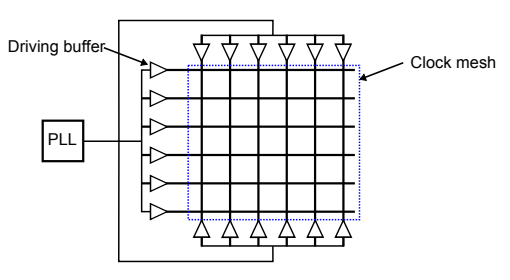
\includegraphics[scale=0.4]{eldar_mesh}
	\end{columns}
 
\end{frame}


\begin{frame}{Avoidance of Mismatch}
  % - A title should summarize the slide in an understandable fashion
  %   for anyone how does not follow everything on the slide itself.

    \begin{itemize}
        \item[--]
            Attempts to fix mismatch: centralised/decentralised skew compensation.
        \item[--]
            Centralised: main controller checks local skew \& tunes forward path.
        \item[--]
            Decentralised: local controller tunes its own clock path.
        \item[--]
            Both methods suffer from high power consumption.
        \item[--]
        \begin{columns}        	
        	\column{0.4\linewidth}
        	\flushleft
            PLL network:
             \begin{itemize}
	            \item[]
	           	 	PLLs generate clock in an area of chip.
	            \item[]
	            	Synced via lower freq. error signal between oscillators.
	            \item[]
	            	Error signals of neighbours used for phase sync.
            \end{itemize}
        	\column{0.35\linewidth}
        	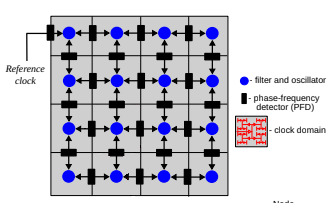
\includegraphics[scale=0.55]{network_ccic2013}
        \end{columns}
     \end{itemize}   
 
\end{frame}
\section*{ADPLL Network}

\begin{frame}{ADPLL Network}
  % - A title should summarize the slide in an understandable fashion
  %   for anyone how does not follow everything on the slide itself.

    \begin{itemize}
        \item[--]
            \textbf{Reminder:} A Phase Lock Loop outputs a signal phase synchronised with a multiple of the reference.
            \begin{center}
            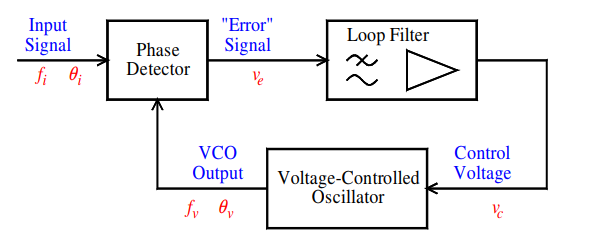
\includegraphics[scale=0.3]{mulkeen_pll}
            \end{center}
        \item[--]
            ADPLL:
            \begin{itemize}
	        \item[]
	            Uses only digital blocks (Digital Loop Filter etc.)
	        \item[]
	           Number controller oscillator $\rightarrow$ quantised frequency
	        \item[]
	            Digital phase detector output $\rightarrow$ quantised phase detection
        	\end{itemize}
    	\item[--]
    		Example node:
			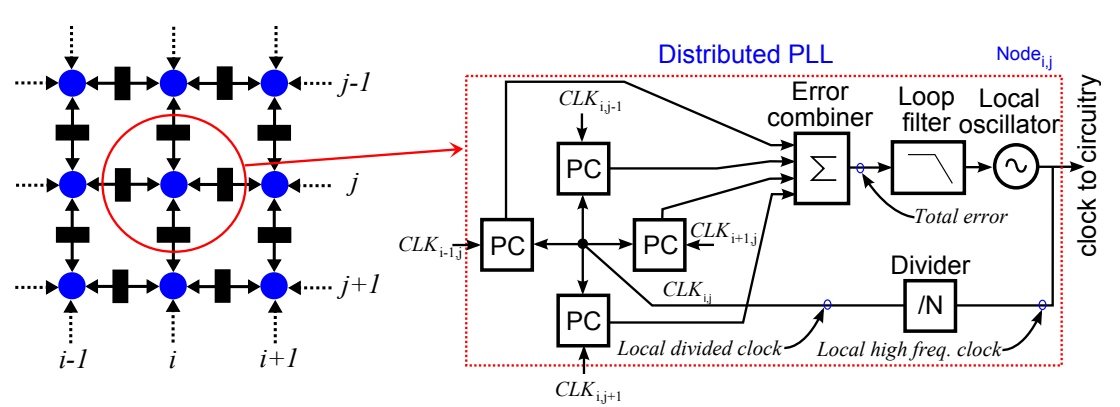
\includegraphics[scale=0.3]{eldar_node}
    \end{itemize}
\end{frame}

\begin{frame}{Network on an FPGA}
  % - A title should summarize the slide in an understandable fashion
  %   for anyone how does not follow everything on the slide itself.

    \begin{itemize}
        \item[--]
            An FPGA is the optimum platform for rapid physical prototyping/limited validation.
        \item[--]
        	Enables low cost testing of potential network architectures and control schemes.
        	%TODO ask Elena for a good thing to say here
        \item[--]
        	FPGA implementation brings with it some challenges:
        	\begin{itemize}
        		\item[]
        			Restriction placed on available hardware. No gates, only LUTs.
        		\item[]
        			No delay lines for time-digital converter.
        		\item[]
        			Frequency must be downscaled to MHz from GHz region.
        		\item[] 
        			Synchroniser to avoid metastability in phase detector sets phase difference step size.
        		
        	\end{itemize}
    \end{itemize}
 
\end{frame}

\begin{frame}{My ADPLL}
  % - A title should summarize the slide in an understandable fashion
  %   for anyone how does not follow everything on the slide itself.
 	%\begin{columns}
 	\begin{center}
 		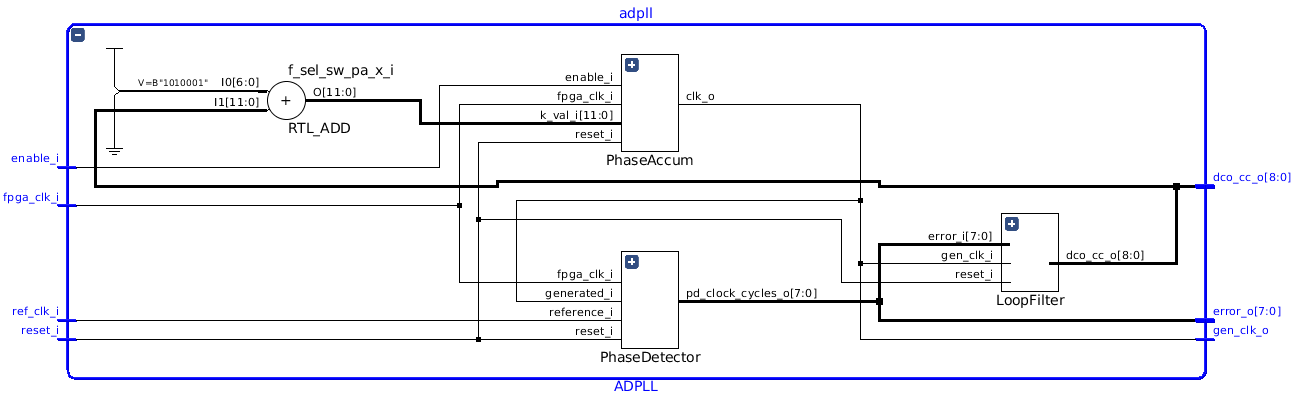
\includegraphics[scale=0.25]{../ADPLL_RTL_VIVADO}
 	\end{center}
		
	\begin{itemize}
		\item[--]
			2 different oscillators made - Inverter Chain \& Phase Accumulator.
		\item[--]
			5 MHz bias point, FPGA clock at 258 MHz.
		\item[--]
			12 bit Phase Accumulator, 9 LSB control code, $60.975$ kHz frequency step.
		\item[--]
			8 bit Phase Detector, resolution of $6.975^\circ$ at 5 MHz.
		\item[--]
			9 bit PI Loop Filter, $k_p=1$ \& $k_i=0.125$. %from paper as a viable value
	\end{itemize}
	%\end{columns}
\end{frame}

\section*{Measurements}
\begin{frame}{Simulations}
% - A title should summarize the slide in an understandable fashion
%   for anyone how does not follow everything on the slide itself.

\begin{itemize}
	\item
	Why use this?
\end{itemize}

\end{frame}

\begin{frame}{Measurements}
  % - A title should summarize the slide in an understandable fashion
  %   for anyone how does not follow everything on the slide itself.

    \begin{itemize}
        \item
            Why use this?
    \end{itemize}
 
\end{frame}

\section*{Future Work}

\begin{frame}{Future Work}
  % - A title should summarize the slide in an understandable fashion
  %   for anyone how does not follow everything on the slide itself.

    \begin{itemize}
        \item
            Why use this?
    \end{itemize}
 
\end{frame}

\section*{Summary}

\begin{frame}{Summary}

  % Keep the summary *very short*.
  \begin{itemize}
  \item
    The \alert{first main message} of your talk in one or two lines.
  \item
    The \alert{second main message} of your talk in one or two lines.
  \item
    Perhaps a \alert{third message}, but not more than that.
  \end{itemize}

  % The following outlook is optional.
  \vskip0pt plus.5fill
  \begin{itemize}
  \item
    Outlook
    \begin{itemize}
    \item
      Something you haven't solved.
    \item
      Something else you haven't solved.
    \end{itemize}
  \end{itemize}
\end{frame}



% All of the following is optional and typically not needed.
\appendix
\section<presentation>*{\appendixname}
\subsection<presentation>*{For Further Reading}

\begin{frame}[allowframebreaks]
  \frametitle<presentation>{For Further Reading}

  \begin{thebibliography}{10}

  \beamertemplatebookbibitems
  % Start with overview books.

  \bibitem{Author1990}
    A.~Author.
    \newblock {\em Handbook of Everything}.
    \newblock Some Press, 1990.


  \beamertemplatearticlebibitems
  % Followed by interesting articles. Keep the list short.

  \bibitem{Someone2000}
    S.~Someone.
    \newblock On this and that.
    \newblock {\em Journal of This and That}, 2(1):50--100,
    2000.
  \end{thebibliography}
\end{frame}


\end{document}
